\subsection{Kiến trúc Đặc vụ Học tăng cường (Double DQN Architecture)}
\label{sec:5_5}

Sau khi được tiêm "bản năng" từ Trạm tiền huấn luyện, Đặc vụ (Agent) chính thức bước vào Môi trường Học tăng cường (Gymnasium Environment). Tại đây, bài toán dự báo kẹt xe được định hình lại thành một quá trình Ra quyết định Markov (Markov Decision Process - MDP).

\begin{figure}[H]
    \centering
    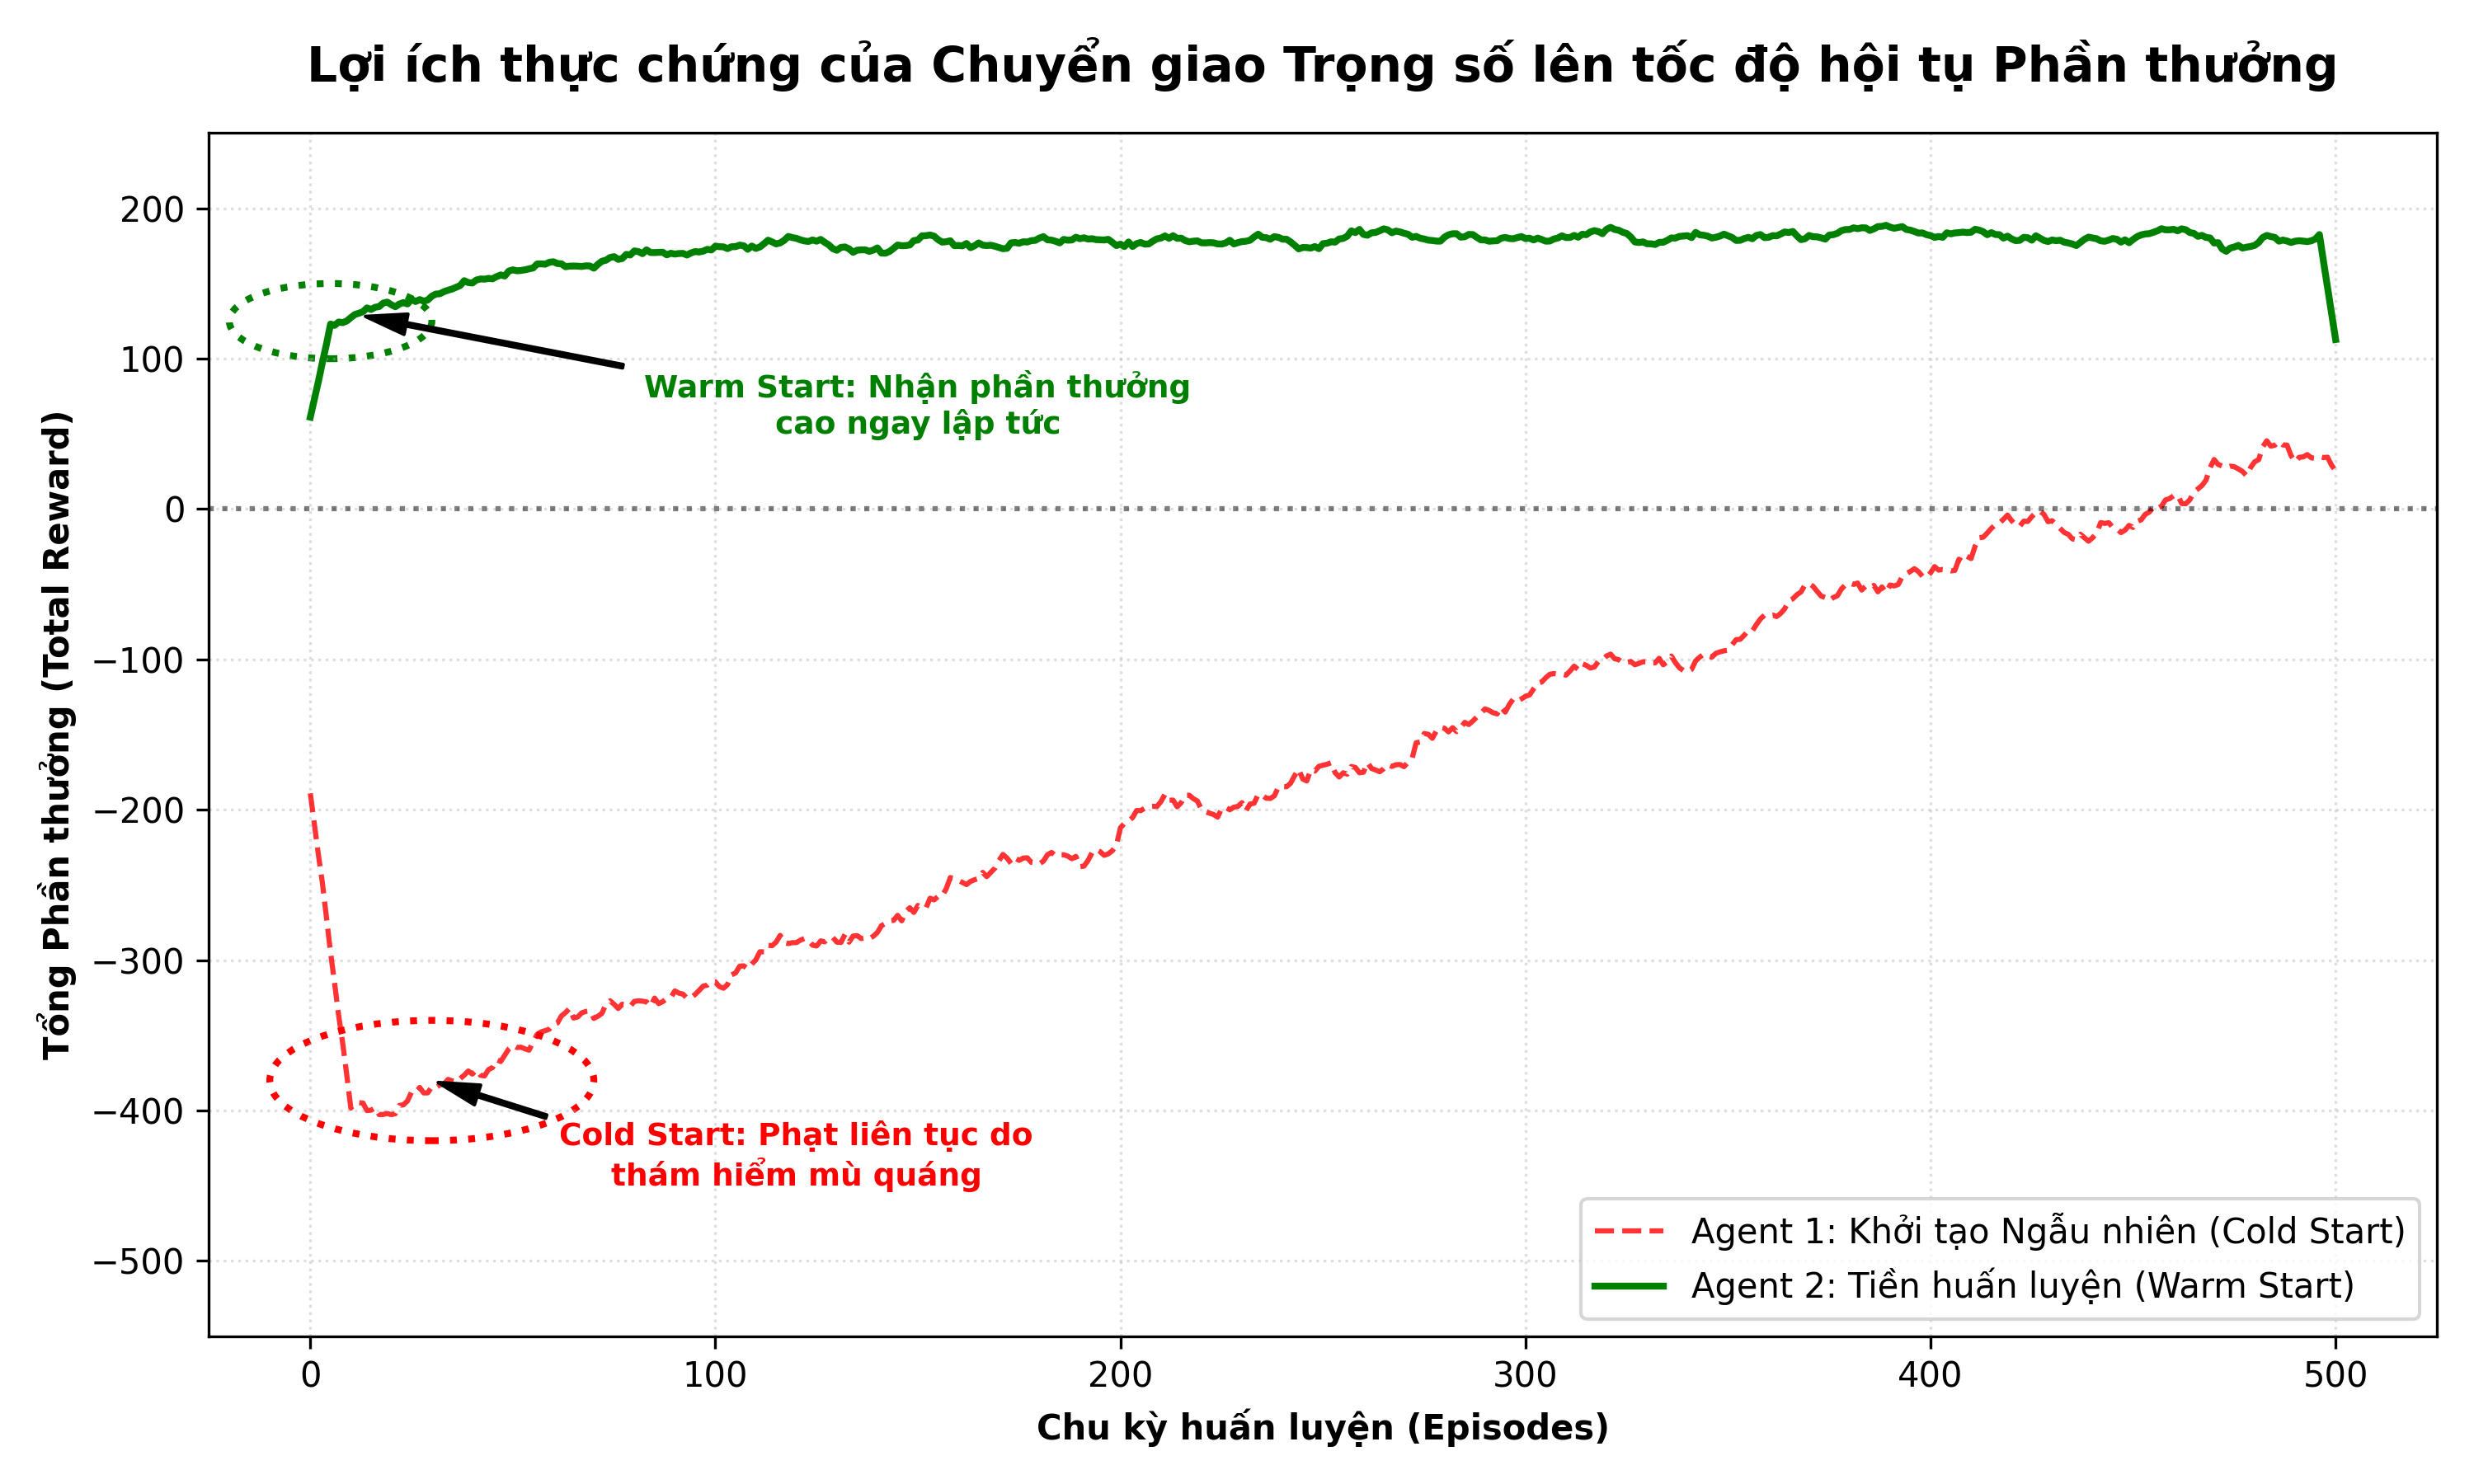
\includegraphics[width=0.8\textwidth]{Images/CH5/17.png}
    \vspace{12pt}
    \caption{Lợi ích thực chứng của Chuyển giao Trọng số lên tốc độ hội tụ Phần thưởng}
    \label{fig:5_17}
\end{figure}

\subsubsection{Lựa chọn thuật toán Double DQN (DDQN)}

Trong hệ sinh thái các thuật toán Học tăng cường Sâu, việc lựa chọn thuật toán phải tuân thủ nghiêm ngặt đặc tính của Không gian hành động (Action Space). Vì hệ thống cần phân loại trạng thái giao thông thành 6 mức độ rời rạc (Discrete classes từ 0 đến 5), các thuật toán dựa trên hàm giá trị (Value-based methods) tỏ ra ưu việt hơn so với các phương pháp tối ưu chính sách liên tục.

Tuy nhiên, thay vì sử dụng mạng Q-Learning sâu truyền thống (Standard DQN), đồ án quyết định triển khai kiến trúc \textbf{Double Deep Q-Network (DDQN)}. Quyết định này xuất phát từ việc khắc phục một lỗ hổng toán học chí mạng:

\paragraph{a. Lỗ hổng của DQN truyền thống: Hội chứng Đánh giá vượt mức (Overestimation Bias)} \mbox{} \\
Trong thuật toán DQN tiêu chuẩn, DQN sử dụng cùng một bộ trọng số mạng $\theta_t$ để thực hiện đồng thời hai nhiệm vụ: (1) Lựa chọn hành động tốt nhất và (2) Đánh giá giá trị (Q-value) của hành động đó.

Do môi trường giao thông chứa lượng lớn nhiễu ngẫu nhiên, các ước lượng Q-value ban đầu thường không chính xác. Việc liên tục lấy giá trị cực đại $\max$ sẽ khiến các sai số dương (positive noise) bị tích lũy qua từng vòng lặp. Hậu quả là Agent rơi vào trạng thái \textbf{"Ảo tưởng giá trị" (Overestimation Bias)}: Nó đánh giá quá cao phần thưởng của một số hành động nhất định, dẫn đến chính sách hội tụ sai lệch và thất bại trong việc phát hiện thảm họa.

\paragraph{b. Giải pháp của Double DQN: Tách biệt quyền lực (Decoupling Selection and Evaluation)} \mbox{} \\
Để triệt tiêu hội chứng ảo tưởng này, kiến trúc DDQN phân tách quá trình tính toán thành hai mạng Nơ-ron độc lập, chia sẻ cùng cấu trúc nhưng khác biệt về trọng số:
\begin{enumerate}
    \item \textbf{Mạng Chính (Policy Network - $\theta$):} Đóng vai trò là "Người ra quyết định". Nó phân tích trạng thái tiếp theo $S_{t+1}$ và tìm ra hành động $a^*$ có Q-value cao nhất.
    \item \textbf{Mạng Đích (Target Network - $\theta^-$):} Đóng vai trò là "Ban giám khảo". Nó tiếp nhận hành động $a^*$ do Mạng Chính đề xuất, và đưa ra đánh giá khách quan về giá trị Q thực sự của hành động đó.
\end{enumerate}

\paragraph{c. Tác dụng đối với hệ thống dự báo giao thông} \mbox{} \\
Sự "tách biệt quyền lực" này hoạt động như một cơ chế kiểm chứng chéo (Cross-validation). Nếu Mạng Chính bị nhiễu và đề xuất một dự báo sai lệch (như bỏ lọt kẹt xe Mức 5), Mạng Đích (với bộ trọng số được cập nhật chậm hơn và ổn định hơn) sẽ đánh giá lại hành động đó, trả về một Q-value thấp, từ đó dập tắt sự ảo tưởng của Agent. Kỹ thuật này giúp đường cong Loss ổn định hơn và giữ cho Agent duy trì sự cảnh giác cao độ trước các tín hiệu thảm họa.

\begin{figure}[H]
    \centering
    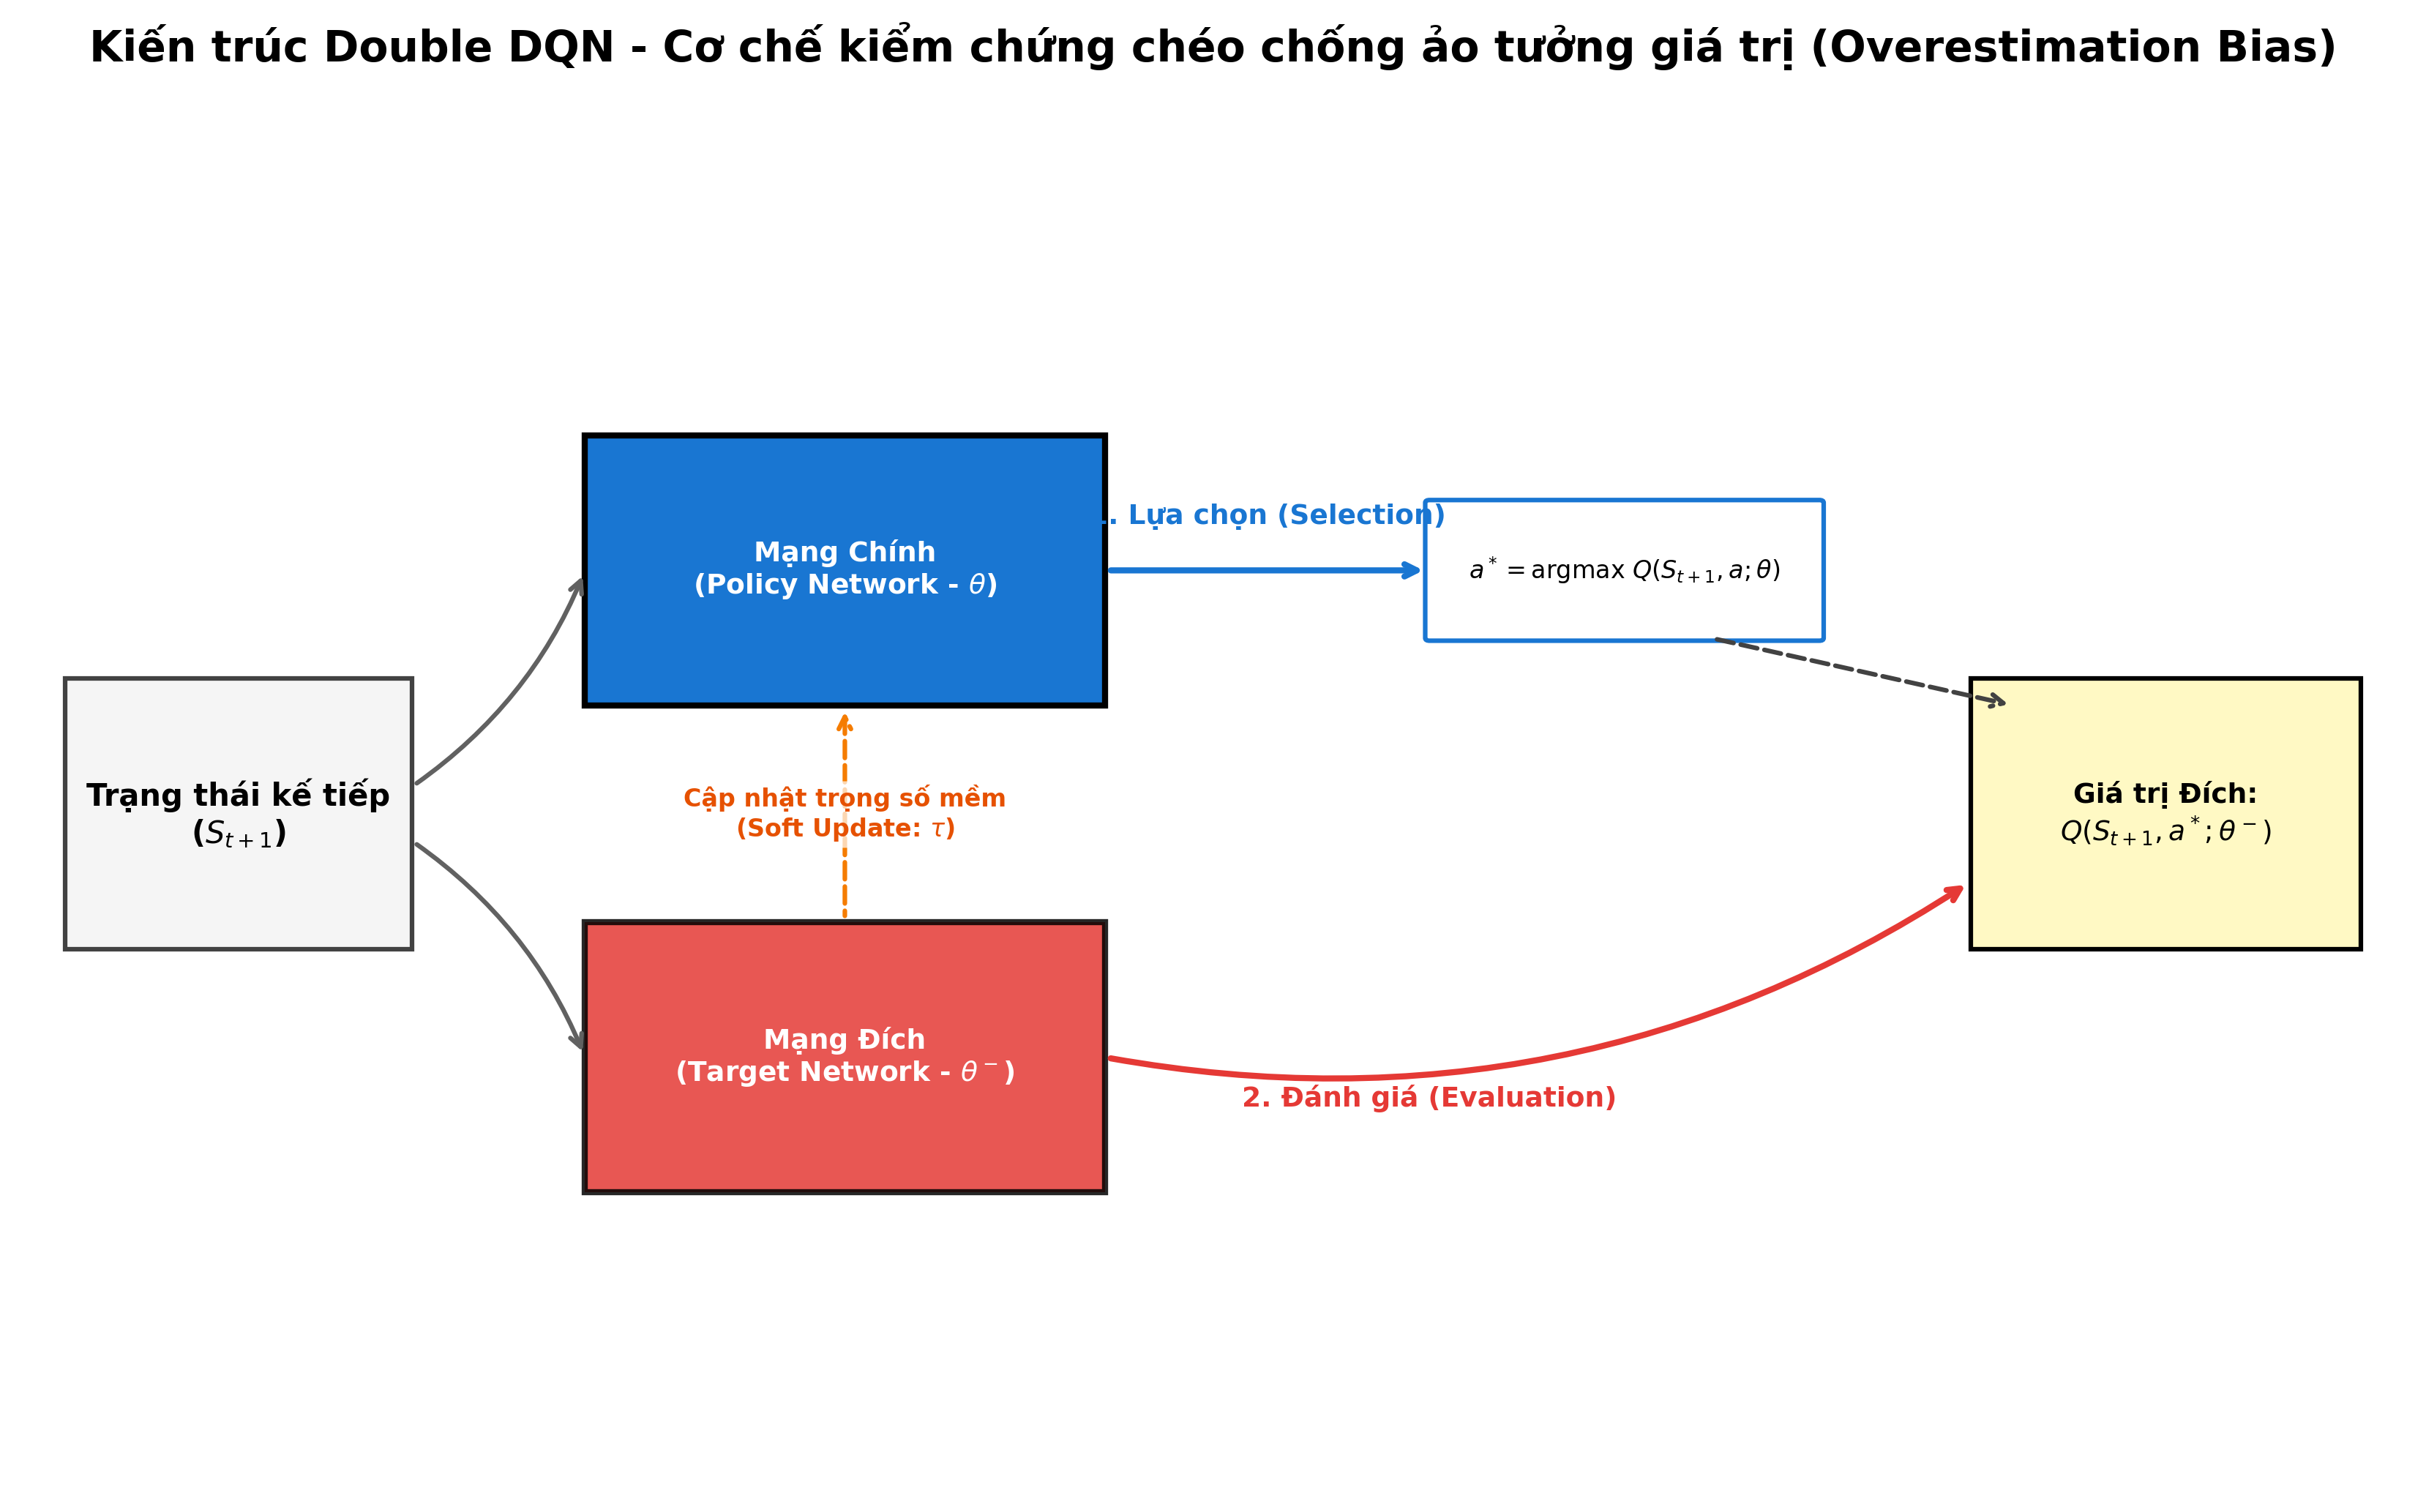
\includegraphics[width=0.8\textwidth]{Images/CH5/18.png}
    \vspace{12pt}
    \caption{Kiến trúc Double DQN - Cơ chế kiểm chứng chéo}
    \label{fig:5_18}
\end{figure}

\subsubsection{Cấu trúc mạng Q-Network và Siêu tham số Huấn luyện}

\paragraph{a. Kiến trúc Q-Network Đa phương thức (Multi-modal Architecture)} \mbox{} \\
Đặc vụ sử dụng một mạng Nơ-ron sâu (DNN) làm hàm xấp xỉ giá trị (Value Function Approximator). Kiến trúc của mạng Q-Network được thiết kế kế thừa và đồng nhất hoàn toàn với mô hình Baseline, sử dụng cấu trúc \textbf{Đa nhánh (Multi-branch)} để xử lý các luồng dữ liệu dị đồng nhất từ môi trường giao thông:
\begin{itemize}
    \item \textbf{Nhánh Dynamic:} Sử dụng các khối LSTM để trích xuất quán tính và sự biến thiên của chuỗi thời gian (vận tốc, độ trễ).
    \item \textbf{Nhánh Categorical:} Sử dụng tầng Embedding để giải mã ngữ cảnh không gian (ID đoạn đường, Phường/Xã).
    \item \textbf{Nhánh Static:} Dùng mạng FNN xử lý các đặc tính hình học không đổi của mạng lưới.
\end{itemize}
Toàn bộ các đặc trưng này hội tụ về các tầng Fully Connected (FC) cuối cùng. Thay vì xuất ra xác suất của các nhãn, lớp output của mạng Q-Network xuất ra một vector chứa $6$ giá trị Q (Q-values), tương ứng với $6$ mức độ kẹt xe.

\paragraph{b. Tối ưu hóa xấp xỉ giá trị với Huber Loss (Smooth L1 Loss)} \mbox{} \\
Trong các bài toán hồi quy hoặc xấp xỉ hàm giá trị của RL, Mean Squared Error (MSE) thường là hàm mất mát mặc định. Tuy nhiên, đồ án đã loại bỏ MSE và quyết định sử dụng \textbf{Huber Loss (Smooth L1 Loss)}.
\begin{itemize}
    \item \textbf{Điểm yếu của MSE:} Hàm MSE bình phương sai số ($x^2$). Nếu có một giá trị nhiễu lớn xuất hiện, MSE sẽ khuếch đại sai số này lên theo cấp số nhân, tạo ra một gradient khổng lồ làm "nổ" trọng số mạng (Exploding Gradient).
    \item \textbf{Sự ưu việt của Huber Loss:} Huber Loss hoạt động như một hàm lai. Đối với các sai số nhỏ, nó cư xử như MSE giúp hội tụ mượt mà. Nhưng đối với các sai số lớn, nó chuyển sang hoạt động như Mean Absolute Error (MAE). Nhờ đó, Huber Loss tự động "cắt gọt" các gradient do nhiễu cảm biến gây ra, giúp mạng Q-Network duy trì sự ổn định tuyệt đối.
\end{itemize}

\paragraph{c. Cấu hình Siêu tham số cốt lõi (Core Hyperparameters Tuning)} \mbox{} \\
Để dẫn dắt Agent hội tụ về một chính sách tối ưu, hệ thống thiết lập:
\begin{enumerate}
    \item \textbf{Hệ số chiết khấu (Discount Factor) $\gamma = 0.99$:} Việc đặt $\gamma$ tiệm cận $1$ bắt buộc Đặc vụ phải có tầm nhìn cực kỳ dài hạn (Long-term Vision), xem xét tác động chuỗi của hành động dự báo hiện tại lên các diễn biến giao thông trong $2-3$ giờ tới.
    \item \textbf{Dung lượng Bộ nhớ Kinh nghiệm (Replay Buffer Size) $= 100.000$:} Giúp hệ thống lưu trữ được một lượng lịch sử đủ dài, phá vỡ sự tương quan chuỗi thời gian giữa các bước liên tiếp.
    \item \textbf{Kích thước Lô (Batch Size) $= 64$:} Điểm cân bằng lý tưởng (Sweet spot) giữa hiệu suất tính toán của GPU và phương sai của Gradient.
\end{enumerate}

\subsubsection{Thiết kế Hàm Phần thưởng (Reward Shaping) - "Linh hồn" của sự thông minh}

Nếu Mạng Nơ-ron là "thể xác" và bộ nạp trọng số là "bản năng", thì Hàm phần thưởng (Reward Function) chính là "linh hồn" định hình nên nhân cách và sự thông minh của Đặc vụ.

\paragraph{a. Triết lý thiết kế: Tối ưu hóa hướng an toàn với Phạt không đối xứng (Asymmetric Penalty)} \mbox{} \\
Trong các bài toán dự báo chuẩn, các hàm đánh giá thường có tính đối xứng: Lỗi dự báo cao hơn thực tế (Over-prediction) và lỗi dự báo thấp hơn thực tế (Under-prediction) bị phạt như nhau. Tuy nhiên, khi áp dụng vào một hệ thống Cảnh báo sớm giao thông, tính đối xứng này trở nên cực kỳ nguy hiểm.
\begin{itemize}
    \item \textbf{Báo động giả (Over-prediction):} Hệ thống dự báo kẹt xe nhưng thực tế đường thông thoáng. Người dùng có thể hơi phiền lòng, nhưng rủi ro tổn thất là bằng không.
    \item \textbf{Bỏ lọt thảm họa (Under-prediction):} Hệ thống báo đường thông thoáng nhưng thực tế là một vụ kẹt xe vỡ trận. Người dùng đi vào và mắc kẹt hàng giờ. Sự cố này sẽ lập tức phá hủy hoàn toàn niềm tin của người dùng.
\end{itemize}
Xuất phát từ triết lý "Thà báo nhầm còn hơn bỏ sót", đồ án xây dựng một Hàm phần thưởng phi tuyến tính và \textbf{Không đối xứng (Asymmetric Reward Shaping)} nhằm định hướng Agent hình thành một "Trực giác an toàn" (Safety Intuition).

\paragraph{b. Cơ chế Thưởng/Phạt chi tiết của Ma trận Trạng thái} \mbox{} \\
Hàm phần thưởng $R(y, \hat{y})$ được thiết kế với 4 tầng logic khắt khe:
\begin{enumerate}
    \item \textbf{Thưởng chuẩn xác phân tầng (Stratified Match Bonus):} Khi Đặc vụ dự đoán đúng hoàn toàn ($y = \hat{y}$), nó sẽ nhận được phần thưởng dương (15 điểm cho lớp 0-2 và 10 điểm cho lớp 3-5).
    \item \textbf{Khoan dung với Sai lệch gần (Near Miss Tolerance):} Nếu Agent dự báo lệch đúng 1 cấp ($|\hat{y} - y| = 1$), hệ thống chỉ trừ một mức phạt rất nhẹ là \textbf{-1 điểm}. Cơ chế này tạo ra một vùng đệm linh hoạt, giúp Agent không bị "trừng phạt oan" bởi các nhiễu loạn ranh giới nhỏ.
    \item \textbf{Phạt sai lệch xa (Far Miss Penalty):} Khi độ chênh lệch cấp độ tăng lên ($|\hat{y} - y| \ge 2$), mức phạt bắt đầu gia tăng tuyến tính và lũy tiến (từ -6, -9, đến \textbf{-17 điểm}). Logic này ép mạng Q-Network phải học và tôn trọng tính thứ bậc của không gian trạng thái.
    \item \textbf{PHẠT SINH TỬ (Severe Mismatch / Fatal Penalty):} Đây là "bức tường thép" mang tính sống còn: Nếu thực tế xảy ra kẹt xe thảm họa (Lớp 4, Lớp 5) nhưng Agent lại chủ quan dự báo là đường thông thoáng (Lớp 0, Lớp 1), mức phạt sẽ lao dốc xuống đáy, dao động từ \textbf{-19 điểm đến -25 điểm}.
\end{enumerate}
Mức phạt tàn khốc này áp đảo hoàn toàn mọi điểm thưởng tích lũy, tạo ra một nỗi "sợ hãi" toán học, ép Đặc vụ thà dự báo nhầm còn hơn bỏ sót thảm họa.
